\documentclass[thesis.tex]{subfiles}
\begin{document}

\chapter{SpeedCam}\label{chap:basics}

The REAL stuff. All your precious work written down for the benefit of humanity.

\section{Overview}

\section{Detection scheme}
This part will contain the description about the detection scheme. It will outline how to detect a greedy user and provide a detailed overview of its functionality.

\subsection{Basic idea}
The task of the detection scheme is to identify a greedy AS inside an ISD using multi-path connections. 

A central unit inside the ISD will be able to start an inspection and inspect ASes bandwidth usage. This is done by a core AS, which is called \textbf{inspector}. 

The inspector will randomly choose ASes inside its ISD to measure the bandwidth. The chosen ASes are called \textbf{speed cam}. They will collect for a certain amount of time the metrics and aggregate them over time. When the duration is to end, the speed cams will sent the data to the inspector.

When the inspector received the data of all speed cams, he will decide, which user is greedy and who are not. The decision process will be explained in later parts of this work.


\begin{figure}[h]
    \begin{subfigure}{.32\linewidth}
        \centering
        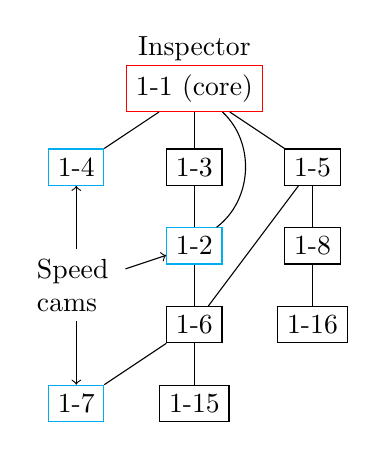
\begin{tikzpicture}
        \node (inspector) at (0, 0.5) {Inspector};
        \node[shape=rectangle,draw=red] (1-1) at (0,0) {1-1 (core)};
        \node[shape=rectangle,draw=cyan] (1-2) at (0,-2) {1-2};
        \node[shape=rectangle,draw=black] (1-3) at (0,-1) {1-3};
        \node[shape=rectangle,draw=cyan] (1-4) at (-1.5,-1) {1-4};
        \node[shape=rectangle,draw=black] (1-5) at (1.5,-1) {1-5};
        \node[shape=rectangle,draw=black] (1-6) at (0,-3) {1-6};
        \node[shape=rectangle,draw=cyan] (1-7) at (-1.5,-4) {1-7};
        \node[shape=rectangle,draw=black] (1-8) at (1.5,-2) {1-8};
        \node[shape=rectangle,draw=black] (1-15) at (0,-4) {1-15};
        \node[shape=rectangle,draw=black] (1-16) at (1.5,-3) {1-16};
        \node (speedcam) at (-1.5, -2.5) [text width=1cm]{Speed cams};
        
        
        \path[-]	
        (1-1) edge (1-4)
        (1-1) edge (1-3)
        (1-1) edge (1-5)
        (1-1) edge[bend left=50] (1-2)
        (1-2) edge (1-6)
        (1-3) edge (1-2)
        (1-5) edge (1-8)
        (1-5) edge (1-6)
        (1-6) edge (1-7)
        (1-6) edge (1-15)
        (1-8) edge (1-16)
        ;
        
        \path[->]
        (speedcam) edge (1-4)
        (speedcam) edge (1-2)
        (speedcam) edge (1-7);
        \end{tikzpicture}
        \caption{Inspector choose ASes for speed cams}
        \label{fig:main:exampleDetectionSchemeSub1}
    \end{subfigure}%
    \begin{subfigure}{.32\linewidth}
        \centering
        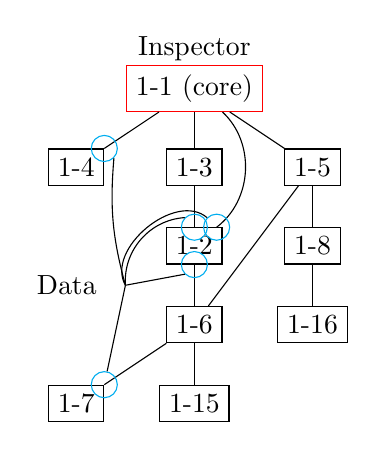
\begin{tikzpicture}
        \node (inspector) at (0, 0.5) {Inspector};
        \node[shape=rectangle,draw=red] (1-1) at (0,0) {1-1 (core)};
        \node[shape=rectangle,draw=black] (1-2) at (0,-2) {1-2};
        \node[shape=rectangle,draw=black] (1-3) at (0,-1) {1-3};
        \node[shape=rectangle,draw=black] (1-4) at (-1.5,-1) {1-4};
        \node[shape=rectangle,draw=black] (1-5) at (1.5,-1) {1-5};
        \node[shape=rectangle,draw=black] (1-6) at (0,-3) {1-6};
        \node[shape=rectangle,draw=black] (1-7) at (-1.5,-4) {1-7};
        \node[shape=rectangle,draw=black] (1-8) at (1.5,-2) {1-8};
        \node[shape=rectangle,draw=black] (1-15) at (0,-4) {1-15};
        \node[shape=rectangle,draw=black] (1-16) at (1.5,-3) {1-16};
        \node (data) at (-1.5, -2.5) [text width=1cm]{Data};
        
        \path[-]		
        (1-1) edge node[shape=circle,draw=cyan, at end] (data1) {} (1-4)    
        (1-1) edge (1-3)
        (1-1) edge (1-5)
        (1-1) edge[bend left=50] node[shape=circle,draw=cyan, at end] (data2) {} (1-2)
        (1-2) edge node[shape=circle,draw=cyan, at start] (data3) {} (1-6)
        (1-3) edge node[shape=circle,draw=cyan, at end] (data4) {} (1-2)
        (1-5) edge (1-8)
        (1-5) edge (1-6)
        (1-6) edge node[shape=circle,draw=cyan, at end] (data5) {} (1-7)
        (1-6) edge (1-15)
        (1-8) edge (1-16)
        ;
        \path[-]
        (data1.south east) edge[bend right=10] (data.east)
        (data2.north west) edge[bend right=80] (data.east)
        (data3.south west) edge (data.east)
        (data4.north west) edge[bend right=45] (data.east)
        (data5) edge (data.east)
        ;
        \end{tikzpicture}
        \caption{Speed cams collect data about traffic}
        \label{fig:main:exampleDetectionSchemeSub2}
    \end{subfigure}%
    \begin{subfigure}{0.32\linewidth}
        \centering
        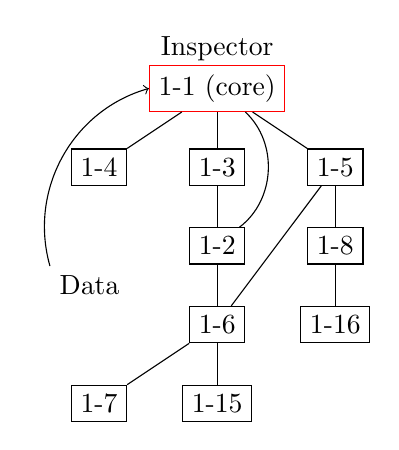
\begin{tikzpicture}
        \node (inspector) at (0, 0.5) {Inspector};
        \node[shape=rectangle,draw=red] (1-1) at (0,0) {1-1 (core)};
        \node[shape=rectangle,draw=black] (1-2) at (0,-2) {1-2};
        \node[shape=rectangle,draw=black] (1-3) at (0,-1) {1-3};
        \node[shape=rectangle,draw=black] (1-4) at (-1.5,-1) {1-4};
        \node[shape=rectangle,draw=black] (1-5) at (1.5,-1) {1-5};
        \node[shape=rectangle,draw=black] (1-6) at (0,-3) {1-6};
        \node[shape=rectangle,draw=black] (1-7) at (-1.5,-4) {1-7};
        \node[shape=rectangle,draw=black] (1-8) at (1.5,-2) {1-8};
        \node[shape=rectangle,draw=black] (1-15) at (0,-4) {1-15};
        \node[shape=rectangle,draw=black] (1-16) at (1.5,-3) {1-16};
        \node (data) at (-1.5, -2.5) [text width=1cm]{Data};
        
        \path[-]	
        (1-1) edge (1-4) 
        (1-1) edge (1-3)
        (1-1) edge (1-5)
        (1-1) edge[bend left=50] (1-2)
        (1-2) edge (1-6)
        (1-3) edge (1-2)
        (1-5) edge (1-8)
        (1-5) edge (1-6)
        (1-6) edge (1-7)
        (1-6) edge (1-15)
        (1-8) edge (1-16)
        ;
        
        \path[->]
        (data.north west) edge[bend left=45] (1-1.west);
        \end{tikzpicture}
        \caption{Speed cams report data to inspector}
        \label{fig:main:exampleDetectionSchemeSub3}
    \end{subfigure}
    \caption{Example of detection scheme}
    \label{fig:main:exampleDetectionScheme}
\end{figure}

The \Cref{fig:main:exampleDetectionScheme} shows an example for the detection scheme. It shows a the ISD 1 and its ASes. In \Cref{fig:main:exampleDetectionSchemeSub1} is the process of choosing speed cams visualized. The ASes 1-2, 1-4 and 1-7 are randomly chosen and now called speed cams. For a certain amount of time, the speed cams collect data about traffic through their border router. This can be seen in \Cref{fig:main:exampleDetectionSchemeSub2}. After the collection is finished, the data is sent to the inspector, which is shown by \Cref{fig:main:exampleDetectionSchemeSub3}.

The following section will explain the details about the selection, the data to collect and to classify the user.

\subsection{Selection process}
This part will explain the process how ASes are selected to be speed cams.

It is obvious that the inspector has to randomly pick ASes at random time slots. If the process were deterministic, then malicious ASes could exploit it. They would use fewer resources at the time of the inspection and so avoid punishment.

It is also important to only inspect, when it is necessary. By limiting the monitoring, fewer resources as the bandwidth or computation time are utilized. One possibility is to start the inspection when a bandwidth is exceeded inside the ISD. This happens when the total currently used bandwidth of a connection is higher than the capacity. Using the method can be too late to avoid the congestion, but it would limit the resource usage. 
It is also important to have a cooldown time between inspection, even if the congestion cannot be solved by punishing greedy user. Otherwise the inspection will be done without an effect.

\todo{Add example graph for that}

Another approach is to prevent such data jams by randomly monitoring ASes throughout the day. This would be done without the urgent need of a bandwidth exceed. This will waste resources but can identify a greedy user before he can disturb other user. 

A mix of both approaches will be investigated by this work. The first investigation will be shorter than the second because of the urgency to identify the source of the congestion. The second one can be done over a longer period for a more accurate result.

\todo{Add obvious impossible approaches: ALways monitor, never monitor}

The necessary amount of speed cams inside a ISD is one interesting question to answer. Fewer speed cams result in a lower resource impact, which is good. But it will also result in a lower precision, which can lead to wrong accusations or missing greedy users.

A pure random amount of ASes is a intuitive answer, but in big ISD with hundreds of ASes only one speed cam will be not enough to measure multi-path bandwidth. An improved version is that the amount is between a certain percentage of the total ASes and the total number itself.

\todo{This should be answered inside experiments or maybe in further works?}

\subsection{Data and metrics}
This part will describe the metrics which are measured and the resulting data which is collected by the inspection.

Each speed cam will collect the same data over the same time period and sent them to the inspector. The data will be aggregated over time, if possible, to minimize the memory consumption of the ASes.

The following list show this metrics:
\begin{easylist}
    \MyListProperties
    # avg. bandwidth usage per AS
    # avg. sent packages per AS
    # avg. received packages per AS
    # requests to path server 
\end{easylist}

The requests to the path server can be used to find the different path an AS uses for its transmissions. 

It is also necessary that the inspector has the complete topology of its ISD. This is used to calculate the percentage of available and used bandwidth by an AS. The topology can be retrieved from the Core AS path server.

\todo{Use work of ? with his buckets to get the values}

\subsection{Classify user}
This part will explain how to distinguish between a greedy and a normal user. This is important to identify a source for a data congestion and the stop it.


One attribute of a greedy user is that he uses more bandwidth than other user constantly. Another attribute is, that it is uses more bandwidth from the network than provide to the network. 

The first attribute can be calculate from the measured data as defined in the previous section. For the second one the work of \todo{add paper about virtual credit} can be used. 
A greedy user uses way more bandwidth than other user. 

\todo{What is the different between a greedy and a normal user?}
\section{Next parts}
\begin{easylist}
    \MyListProperties
        ## Parameters of detection scheme
        ### Frequency
        ### Duration
        ### Sample size
        ## Security
        ### How to prevent lying AS
        ### How to prevent misusing the system(for dDos)
        # Punishment scheme
        ## Overview
        ## Level system for punishment (\textit{Flensburger system})
        ### \textit{Table of different levels and their punishments}
        ### How to get \"points\"
        ### Explain the levels
        ## Enforcement of punishment
        ### Describe responsibility (coreAS or coordinator?)
    \end{easylist}
\subfilebib % Makes bibliography available when compiling as subfile
\end{document}